\documentclass[a4paper,12pt]{article}

\usepackage[utf8]{inputenc}
\usepackage[T1]{fontenc}
\usepackage{color}
\definecolor{grey}{rgb}{0.9,0.9,0.9}
\definecolor{teal}{rgb}{0.0,0.5,0.5}
\definecolor{violet}{rgb}{0.5,0,0.5}
\usepackage[margin=2.5cm]{geometry}
\usepackage{graphicx}
\usepackage[francais]{babel}
\usepackage[babel=true]{csquotes}
\usepackage{listings}

\title{TP3 - Analyse de concepts}
\author{\textsc{Paul Chaignon} - \textsc{Ulysse Goarant}}
\date{\today}

\begin{document}

\maketitle


\section{Système solaire}

\subsection*{Question 1}

Le treillis associé aux planètes est le suivant :

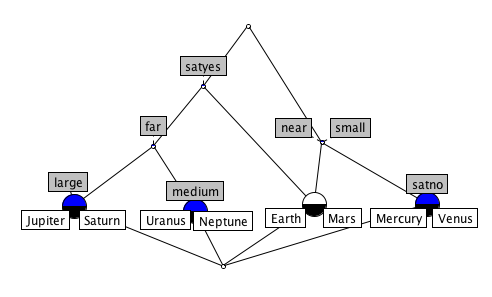
\includegraphics[width=400px]{question1.png}

On peut remarquer qu'une petite planète est toujours proche du soleil (et inversement).
Par contre, une planète éloignée du soleil possède forcément un satellite mais l'inverse n'est pas vrai.


\subsection*{Question 2}

De part sa spécificité, un exemple tel que Pluton modifie fortement la structure du treillis.
Cela est du au fait que dans le concept d'analyse formelle, l'exception a autant de poids que la généralité.


\subsection*{Question 3}

\textit{Show only exact matches} affiche uniquement le comptage des exemples qui possèdent les attributs en intention, alors que \textit{Show all matches} affiche le comptage des exemples possédant simplement et non nécessairement de manière exclusive l'attribut.



\section{\'Echelle conceptuelle}

\subsection*{Question 4}

La taille des disques durs a une échelle et des attributs de type numérique (continu). Les types de bus système ont une échelle et des attributs de type nominal. Les moyens de distribution ont une échelle de type nominal et des attributs de type booléen.



\section{Recensement américain : implications-règles d'association}

\subsection*{Question 5}

On constate que la base d'implication est contenue dans les règles extraites.


\subsection*{Question 6}

Il n'est bien sûr pas visuellement exploitable.



\section{Base de comics gérée avec Camelis}

\subsection*{Question 8}

Le contexte contient 628 objets qui possèdent 7 attributs (desinateur, éditeur, genre, nom de la série, note sur 5, scénariste et source).


\subsection*{Question 9}

En utilisant la navigation dans la propriété \textit{éditeur}, on trouve que le nombre de séries par éditeur varie de 11 à 72 selon ce dernier.
Selon la même méthode appliquée à la propriété \textit{dessinateur}, on détermine que le dessinateur ayant le plus de comics est Corben (Richard).


\subsection*{Question 10}

Pour connaître les dessinateurs et les scénaristes des comics les plus appréciés, il faut sélectionner les attributs \textit{Dessinateur}, \textit{Scénariste} et \textit{Note /5 is 4 (2avis)} ou alors de taper la requête \textit{"Scénariste" ? and "Note /5" is  "4 (2avis)" and Dessinateur ?}. Peter Bagge fait, par exemple, partie des dessinateurs des comics préférés des lecteurs.

Pour connaître les dessinateurs et scénaristes des comics les moins appréciés, il faut sélectionner \textit{Note /5 is 1} au lieu de \textit{Note /5 is 4 (2avis)}.


\subsection*{Question 11}

Pour savoir quelles sont les séries de comics qui contiennent \textit{Batman} dans leur titre et qui ne sont pas éditées par Panini Comics ni Semic, il faut utiliser la requête : \textit{"Nom série" contains "Batman" and not Editeur is "Semic" and not Editeur is "Panini Comics"}. On trouve alors que \textit{Batman – Année 1} et \textit{Batman – Cris dans la nuit} comme résultats.


\subsection*{Question 12}

\`A l'aide de la requête \textit{"Nom série" ? and not Genre ?}, on trouve que textit{Blondie} n'a pas de genre.


\subsection*{Question 13}

On utilise la requête \textit{"Nom série" contains "Blanche" or "Nom série" contains "noire" or "Nom série" contains "mort" or "Nom série" contains "vie") and not or "Nom série" contains "une" and not or "Nom série" contains "une"}. On obtient alors par exemple \textit{\`A l'ombre des tours mortes}, \textit{Mon dernier jour au Vietnam}, \textit{Mort@17}, etc.


\end{document}